\documentclass[journal]{IEEEtran}

\usepackage[utf8]{inputenc}
\usepackage[T1]{fontenc}
\usepackage{cite}
\usepackage{url}
\usepackage{graphicx}
\usepackage{booktabs}
\usepackage{amsmath}
\usepackage[hidelinks]{hyperref}

% Marcador visible para lo que falta. Antes de la version final: buscar "TODO".
\newcommand{\todo}[1]{\textbf{[TODO: #1]}}

\begin{document}

\title{False Sharing and Scalability in Multicore Processors: Impact of Cache-Line Data Layout on Parallel Performance}

\author{Walter Alfaro, Allan Arrieta}

\markboth{Arquitectura de Computadores I, II Semester 2026}%
{False Sharing and Scalability in Multicore Processors}

\maketitle

% TODO (preliminar): ajustar el abstract para mencionar el simulador MESI y la
% lectura critica de las fuentes. Sigue sin numeros hasta tener mediciones.
\begin{abstract}
Modern multicore processors keep private caches coherent at the granularity of a
cache line, typically 64 bytes, rather than individual variables. When threads
running on different cores write to independent variables that happen to reside
in the same cache line, the coherence protocol forces the line to migrate
repeatedly between cores, even though no data is logically shared. This
phenomenon, known as false sharing, generates invalidation traffic and
cache-to-cache transfers that can severely limit the scalability of parallel
programs and is a recurring source of performance regressions in large systems
such as the Linux kernel. This paper investigates how the distribution of
variables across cache lines affects the performance of a parallel program on a
hybrid x86-64 Intel Core i7-1260P (Alder Lake) processor, which combines
performance and efficiency cores. We study a microbenchmark in which each
thread, pinned to a dedicated core, updates its own independent counter,
comparing a layout where the counters are
stored contiguously against layouts in which they are separated through
alignment and padding, as well as per-thread accumulation. The analysis relates
the observed execution time and scalability with the number of threads to the
behavior of the MESI-family coherence protocol, and uses hardware performance
counters and the Linux \texttt{perf c2c} tool to identify contended cache lines
through HITM (load hit in a modified line) events. In addition, the memory and
cache-capacity overhead introduced by padding is quantified, together with the
mitigation strategies documented by the Linux kernel community, in order to
characterize the trade-off between coherence-traffic reduction and memory
footprint and to derive practical guidelines for cache-aware data layout.
\end{abstract}

\begin{IEEEkeywords}
False sharing, cache coherence, MESI, multicore processors, cache line, padding, performance analysis, perf c2c, Linux kernel.
\end{IEEEkeywords}

% =====================================================================
\section{Introduction}
\label{sec:intro}
% =====================================================================
% Objetivo: motivar el problema y plantear las preguntas. ~0.75 columnas.

\IEEEPARstart{P}{arallel} programs are expected to run faster as more cores are
added. A well-known obstacle to this expectation is \emph{false sharing}: threads
that never touch each other's data can still slow each other down when their
data happen to share a cache line~\cite{torrellas1994false,tang2023kernel}.
Because the effect depends on memory layout rather than on the algorithm, it is
invisible in the source code and is usually discovered only through
profiling~\cite{mario2016c2c,liu2011sheriff}.

\todo{1 parrafo: por que importa hoy (kernel, servidores, laptops hibridas).
Citar la doc del kernel como fuente del problema, no como prueba de magnitud.}

Most of the guidance on false sharing comes from a small group of sources:
processor vendors, the developers of the detection tools, and research
prototypes evaluated by their own authors. Rather than taking that guidance at
face value, this paper treats each recommendation as a claim to be tested. We
pose three questions:
\begin{enumerate}
  \item \textbf{RQ1:} How much does placing independent counters in the same
        cache line degrade performance and scalability on a contemporary
        hybrid laptop processor?
  \item \textbf{RQ2:} Which commonly cited claims about false sharing
        (magnitude of the slowdown, need for 128-byte padding, reliability of
        HITM-based detection) hold under our model and measurements, and which
        depend on the context in which their sources were produced?
  \item \textbf{RQ3:} What does mitigation cost in memory footprint, and when
        is that cost worth paying?
\end{enumerate}

\todo{Contribuciones: (1) simulador MESI propio y abierto; (2) mediciones en
i7-1260P con perf c2c; (3) contraste simulacion vs. hardware; (4) lectura
critica de las fuentes. Ultimo parrafo: organizacion del paper.}

% =====================================================================
\section{Background}
\label{sec:background}
% =====================================================================

\subsection{Coherence at Cache-Line Granularity}
Private caches in a multicore processor are kept coherent by a hardware
protocol. The unit tracked by the protocol is the cache line (64 bytes on
current x86-64 processors~\cite{intel2024opt}), not the individual variable.
Consequently, two variables that reside in the same line are treated by the
hardware as a single shared object~\cite{hennessy2017ca,nagarajan2020primer}.

\subsection{The MESI Protocol}
\todo{Describir los 4 estados (M, E, S, I), las transacciones BusRd, BusRdX y
BusUpgr, y una tabla o diagrama de transiciones. Fuentes: Hennessy--Patterson y
Nagarajan et al. Aclarar que Intel usa una variante (MESIF) y que el detalle
exacto no es publico.}

\subsection{True Sharing vs. False Sharing}
\todo{Definicion formal (Torrellas et al.): un fallo es de false sharing si la
palabra que se invalida no es la que se usa. Condiciones: varios nucleos, misma
linea, al menos una escritura~\cite{tang2023kernel}. Figura: 4 contadores de 8 B
en una linea de 64 B.}

\subsection{Detecting False Sharing with \texttt{perf c2c}}
\todo{Que es un HITM (load que encuentra la linea en estado M en otra cache),
como perf c2c lo muestrea y que reporta (lineas, offsets, nodos/CPUs)
\cite{perf_c2c_man,mario2016c2c}. Anotar desde ya la limitacion: es muestreo y se
basa en loads.}

% =====================================================================
\section{Related Work and Critical Review of Sources}
\label{sec:related}
% =====================================================================
% Seccion clave para la discusion que pidio el profesor. Para cada fuente:
% que afirma, quien la escribe y con que interes, sobre que hardware/carga,
% y como lo ponemos a prueba nosotros. Distinguir: medido / estimado /
% afirmado por el fabricante.

\subsection{What the Sources Claim}
\todo{Resumen breve de cada fuente: Torrellas 1994 (false sharing vs.
localidad espacial y tamano de linea), Liu y Berger 2011 (SHERIFF), doc del
kernel (patrones y mitigaciones), Mario 2016 (perf c2c), manual de Intel
(recomendaciones de layout y prefetcher), Drepper 2007 (costo de coherencia).}

\subsection{Who Wrote Them, and Under What Conditions}
\todo{Para cada fuente, contexto y posible sesgo. Verificar cada punto contra
la fuente antes de afirmarlo.}

\begin{table}[!t]
\caption{Critical Reading of the Main Sources}
\label{tab:sources}
\centering
\footnotesize
\begin{tabular}{@{}p{0.22\columnwidth}p{0.34\columnwidth}p{0.34\columnwidth}@{}}
\toprule
\textbf{Source} & \textbf{Context / possible bias} & \textbf{How we test it} \\
\midrule
Kernel docs~\cite{tang2023kernel} & Written by an Intel engineer; cases from large servers & Magnitude on a 4-P-core laptop \\
Mario~\cite{mario2016c2c} & Co-author of the tool he documents & Detection under few or store-only accesses \\
Intel manual~\cite{intel2024opt} & Vendor document; claims rarely quantified & 64\,B vs.\ 128\,B padding \\
Drepper~\cite{drepper2007memory} & 2007 hardware & Whether costs still hold \\
Torrellas~\cite{torrellas1994false} & Simulated 1990s bus machines & Line-size sweep in our simulator \\
SHERIFF~\cite{liu2011sheriff} & Authors evaluate their own tool & \todo{revisar trabajos posteriores} \\
\bottomrule
\end{tabular}
\end{table}

% =====================================================================
\section{Methodology}
\label{sec:method}
% =====================================================================
% La metodologia debe acordarse con el profesor (guia del curso).

\subsection{Workload}
Each of $N$ threads increments its own 64-bit counter $I$ times. No counter is
ever read or written by another thread, so any coherence traffic between
threads is, by construction, false sharing. Four data layouts are compared:
\begin{itemize}
  \item \textbf{packed:} counters stored contiguously (8\,B apart), so up to
        eight counters share one 64-byte line;
  \item \textbf{padded:} counters separated by a stride $s$ (64 or 128\,B),
        so each occupies its own line;
  \item \textbf{local:} each thread accumulates in a private variable and
        writes the shared array once at the end;
  \item \textbf{shared:} all threads increment the \emph{same} counter
        (true sharing), used as a reference.
\end{itemize}

\subsection{Trace-Driven MESI Simulator}
We implemented a MESI coherence simulator in C (available in the project
repository, \texttt{sim/mesi\_sim.c}). Its model is deliberately simple so that
every result can be traced to a protocol event:
\begin{itemize}
  \item $N$ cores, each with a private set-associative LRU cache;
  \item a single, serialized snooping bus carrying BusRd, BusRdX and BusUpgr
        transactions;
  \item an atomic increment modeled as a read-for-ownership (BusRdX) followed
        by a write, and, alternatively, as a separate load and store;
  \item a per-core clock; at each step the core with the lowest clock issues
        its next access, so contention emerges from timing instead of from a
        fixed interleaving;
  \item an optional \emph{adjacent-line prefetch} that, on a miss, also
        fetches the other line of the aligned 128-byte pair.
\end{itemize}
The simulator counts hits, misses, bus transactions, invalidations,
cache-to-cache transfers from a modified line (the analogue of a HITM),
write-backs, and the memory occupied by the counters. Latencies are model
parameters (Table~\ref{tab:latencies}); a sensitivity sweep over the HITM
latency is also reported.

\begin{table}[!t]
\caption{Simulator Latency Parameters (Cycles at 4.7\,GHz)}
\label{tab:latencies}
\centering
\begin{tabular}{@{}lrl@{}}
\toprule
\textbf{Event} & \textbf{Cycles} & \textbf{Origin} \\
\midrule
Private cache hit & 4 & assumed \\
Locked RMW, line already owned & 18 & calibrated \\
Data from a modified line (HITM) & 47 & calibrated \\
Data from LLC / clean copy & 40 & assumed \\
Main memory & 200 & assumed \\
Upgrade (S$\rightarrow$M) & 30 & assumed \\
\bottomrule
\end{tabular}
\end{table}

The two parameters that dominate the workload were calibrated from our own
measurements on the P-cores (Section~\ref{sec:results}): the cost of an
uncontended locked increment (padded layout, one thread, 3.87\,ns) and the
cost of one line transfer, taken from the slope of the packed layout with four
threads (about 10\,ns per transfer). The remaining values are rough estimates;
they barely affect this workload because, after warm-up, it never misses to
the LLC or to memory. Note that calibrating with data from the same platform
means that agreement at those two points is not an independent validation;
only the predictions for other thread counts and layouts are.

\todo{Aclarar que el bus serializado es una simplificacion: el i7-1260P usa un
ring y una L3 compartida. Explicar por que aun asi el modelo predice el
crecimiento lineal (la linea disputada es una sola: solo un nucleo puede
tenerla en M a la vez).}

Four sweeps are run (\texttt{sim/sweep.sh}): (i) scaling with $N$ for each
layout; (ii) line size versus counter stride; (iii) adjacent-line prefetch with
64-byte and 128-byte padding; and (iv) sensitivity to the HITM latency.

\subsection{Hardware Experiment}
The experiment runs on an Intel Core i7-1260P (Alder Lake) with four
performance cores (P-cores, two hardware threads each, private 1.25\,MiB L2,
up to 4.7\,GHz), eight efficiency cores (E-cores, up to 3.4\,GHz, organized in
two clusters of four that share a 2\,MiB L2) and an 18\,MiB L3 shared by all cores,
under Linux 7.0 with the \texttt{performance} frequency governor. The
benchmark (\texttt{benchmarks/fs\_bench.c}, compiled with GCC 13.3 at
\texttt{-O2}) implements the four layouts of the simulator, with either a
locked increment (\texttt{\_\_atomic\_fetch\_add}, which compiles to
\texttt{lock add}) or a plain \texttt{volatile} increment. Each thread is pinned
to one core, and three groups of cores are compared: one thread per physical
P-core (CPUs 0, 2, 4, 6), four E-cores of one cluster (8--11), and E-cores
split across both clusters (8, 12, 9, 13). Each configuration performs
$5\times10^{7}$ increments per thread and is repeated ten times after one
warm-up run. Contended lines are recorded with \texttt{perf c2c record} for
each layout and core group.

% =====================================================================
\section{Results}
\label{sec:results}
% =====================================================================
% Separar siempre: (A) simulado, (B) medido, (C) comparacion.

\subsection{Simulation}
Table~\ref{tab:simline} shows the simulated cost of an increment with four
threads as a function of the cache-line size and the distance between
counters. The result is binary: whenever two counters fall in the same line,
every increment pays a line transfer; as soon as the distance reaches the line
size, the cost drops to that of an uncontended locked increment. The boundary
moves with the line size, which reproduces in our model the argument of
Torrellas et~al.~\cite{torrellas1994false} that longer lines increase false
sharing.

\begin{table}[!t]
\caption{Simulated ns per Increment, 4 Threads (Packed Counters at Distance $d$)}
\label{tab:simline}
\centering
\begin{tabular}{@{}lrrrrrr@{}}
\toprule
& \multicolumn{6}{c}{\textbf{Distance between counters $d$ (bytes)}} \\
\cmidrule(l){2-7}
\textbf{Line} & 8 & 16 & 32 & 64 & 128 & 256 \\
\midrule
32\,B  & 40.0 & 40.0 & 4.1 & 4.1 & 4.1 & 4.1 \\
64\,B  & 40.0 & 40.0 & 40.0 & 4.1 & 4.1 & 4.1 \\
128\,B & 40.0 & 40.0 & 40.0 & 40.0 & 4.1 & 4.1 \\
256\,B & 40.0 & 40.0 & 40.0 & 40.0 & 40.0 & 4.1 \\
\bottomrule
\end{tabular}
\end{table}

With the adjacent-line prefetch enabled and 64-byte padding, the simulator
records only one to four prefetch-induced HITM events per run (for 2 to 8
threads), all during warm-up. Once each core owns its line in the M state it
never misses again, so the prefetcher is never triggered.
\todo{Mencionar el barrido de sensibilidad (\texttt{hitm\_sensitivity.csv}):
el costo de packed escala linealmente con la latencia HITM supuesta.}

\subsection{Measurements on the i7-1260P}
Fig.~\ref{fig:scaling} shows the cost per increment for each layout and core
group with locked increments. With one thread all layouts except local cost
the same (3.87\,ns on P-cores, 5.32\,ns on E-cores; about 18 cycles in both
cases). With two or more threads, the packed and shared layouts grow roughly
linearly with the thread count, while padded remains almost flat. With four
threads, packed is $8.4\times$ slower than padded on P-cores, $9.2\times$ on
E-cores sharing an L2, and $11.6\times$ on E-cores in different clusters
(Fig.~\ref{fig:slowdown}). Padding to 128 bytes was within 5\% of 64-byte
padding in every configuration and is omitted from the figure. All
configurations were repeated ten times; the coefficient of variation was below
2\% except for the local layout, whose runs last only a few milliseconds.

\begin{figure*}[!t]
\centering
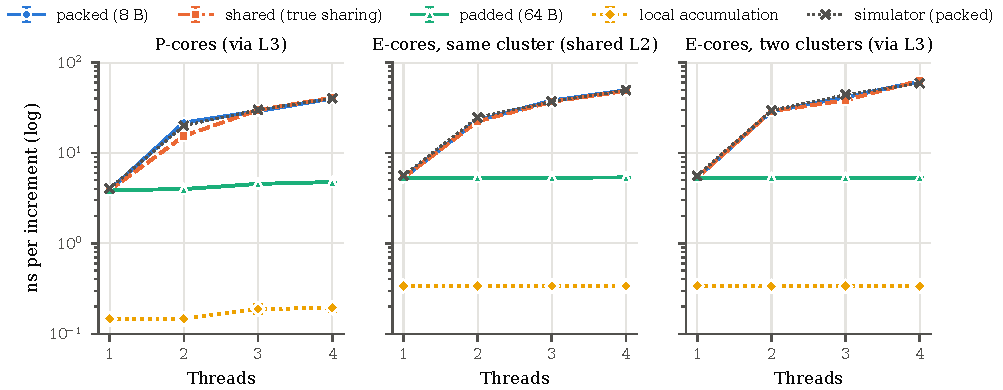
\includegraphics[width=\textwidth]{figures/fig_scaling.pdf}
\caption{Cost per locked increment versus thread count on the i7-1260P (mean
of 10 runs; error bars show one standard deviation, mostly smaller than the
markers). Each panel pins the threads to a different group of cores. The dotted
line is the prediction of our MESI simulator for the packed layout, using the
line-transfer latency calibrated for each group (Table~\ref{tab:latencies}).}
\label{fig:scaling}
\end{figure*}

\begin{figure}[!t]
\centering
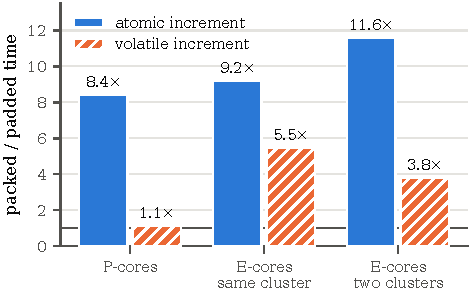
\includegraphics[width=\columnwidth]{figures/fig_slowdown.pdf}
\caption{Slowdown of the packed layout relative to 64-byte padding with four
threads, for locked (\texttt{lock add}) and plain \texttt{volatile} increments.}
\label{fig:slowdown}
\end{figure}

The type of increment changes the picture. With plain \texttt{volatile}
increments (a load, an add and a store, without \texttt{lock}), the packed
layout is only $1.15\times$ slower than padded on P-cores, but $3.8\times$ to
$5.5\times$ slower on E-cores (Fig.~\ref{fig:slowdown}). On a P-core a single
thread completes about one \texttt{volatile} increment per cycle.

Table~\ref{tab:c2c} summarizes the \texttt{perf c2c} recordings. On P-cores,
the tool reports one contended line with 18\,631 HITM samples and shows each
thread writing at a different offset (0x0, 0x8, 0x10, 0x18), exactly the
pattern described by Mario~\cite{mario2016c2c}. Padded and local layouts
produce no HITM. However, the same packed workload on E-cores yields only 54
and 293 HITM samples, and the \texttt{volatile} packed layout yields almost
none on any group.

\begin{table}[!t]
\caption{HITM Samples Reported by \texttt{perf c2c}, 4 Threads}
\label{tab:c2c}
\centering
\begin{tabular}{@{}lrrr@{}}
\toprule
\textbf{Layout} & \textbf{P-cores} & \textbf{E same} & \textbf{E cross} \\
\midrule
packed, atomic   & 18\,631 & 54  & 293 \\
shared, atomic   & 12\,951 & 186 & 97 \\
padded, atomic   & 0       & 0   & 1 \\
local            & 0       & 0   & 0 \\
packed, volatile & 0       & 0   & 20 \\
\midrule
\multicolumn{4}{@{}l}{\emph{Measured slowdown, packed vs.\ padded (atomic)}} \\
& $8.4\times$ & $9.2\times$ & $11.6\times$ \\
\bottomrule
\end{tabular}
\end{table}

\subsection{Simulation vs.\ Hardware}
After calibrating two parameters per core group, the simulator predicts the
packed layout within $\pm7\%$ for two to four threads in all three groups
(Fig.~\ref{fig:scaling}). The fitted line-transfer cost is 47 cycles on
P-cores, 42 cycles between E-cores sharing an L2, and 50 cycles between
E-core clusters. The model fails in two places: it predicts that packed and
shared cost the same, whereas on two P-cores packed is 40\% slower than shared
(21.6 vs.\ 15.4\,ns); and, since it has no store buffer, it cannot reproduce the
near absence of false sharing for \texttt{volatile} increments on P-cores.
\todo{Explicar las dos discrepancias en la Discusion.}

% =====================================================================
\section{Discussion}
\label{sec:discussion}
% =====================================================================
% Aqui se responde RQ2. Cada punto: lo que dice la fuente, lo que vimos,
% y por que podria diferir.

Each subsection below starts from a claim found in the sources, contrasts it
with what we simulated and measured, and states which parts of our explanation
are confirmed and which remain hypotheses.

\subsection{False Sharing Costs as Much as True Sharing}
False sharing is usually presented as a subtler, secondary form of sharing.
Our data do not support that distinction from the point of view of the
hardware. In the simulator, the packed and shared layouts generate exactly the
same sequence of coherence transactions, because the protocol tracks lines and
not words. On the real processor, both layouts cost within 8\% of each other
(within 3\% in five of the six cases) for three and four threads in all core
groups (Fig.~\ref{fig:scaling}). The
practical consequence is that a programmer who removes an obviously shared
variable but leaves independent counters in one line gains nothing.

The only exception is two threads on P-cores, where packed is 40\% slower than
shared (21.6 vs.\ 15.4\,ns). Our model cannot reproduce this, and we have no
confirmed explanation. Possible causes include a different arbitration of
ownership requests when the two threads target different words of the line, or
a difference in how often each core keeps the line for several consecutive
increments. Verifying either would require counters that we have not
collected; we report the discrepancy as an open observation.

\subsection{Does 128-Byte Padding Matter?}
Intel describes a spatial prefetcher that completes the aligned 128-byte pair
of a fetched line~\cite{intel2024opt}, and padding to 128 bytes is often
recommended for that reason. \todo{Verificar la seccion exacta del manual de
Intel que lo dice y si la recomendacion de 128\,B es de Intel o de terceros.}
In our measurements, 128-byte padding was within 5\% of 64-byte padding in
every configuration, and slightly slower in some. The simulator suggests why:
the prefetcher acts only on misses, and once each core owns its padded line in
state M it never misses again, so the neighboring line is fetched at most once
during warm-up (one to four events per run). The recommendation is therefore
not wrong but conditional: it should matter when the contended lines are
repeatedly evicted or re-fetched, for example when the counters are mixed with
other data that miss in the cache. For a tight update loop such as ours, it
doubles the memory cost without a measurable benefit. A vendor manual states
the mechanism but, in our reading, does not quantify when the extra padding pays
off; our results show that it is a workload-dependent decision.

\subsection{The Classic \texttt{volatile} Demonstration Can Hide the Problem}
Many explanations of false sharing, including our own first prototype, use a
loop of \texttt{volatile} increments. On P-cores, this demonstration nearly
fails: packed is only $1.15\times$ slower than padded, while with locked
increments the same layout is $8.4\times$ slower. The difference is that a
\texttt{lock add} must own the line for every single increment, whereas a plain
store can wait in the store buffer. Our hypothesis is that on the P-core the
thread reads its own pending stores (store-to-load forwarding), so its loads
rarely need the line, and the buffered stores drain in bursts whenever the
core obtains ownership, amortizing one transfer over many increments. The fact
that a single P-core thread completes about one dependent \texttt{volatile}
increment per cycle suggests an aggressive forwarding or memory-renaming
mechanism. On E-cores the same code is $3.8\times$ to $5.5\times$ slower when
packed, so the effect is microarchitecture-specific. \todo{Buscar una fuente
sobre store-to-load forwarding / memory renaming en Golden Cove vs.\ Gracemont
para sostener o descartar la hipotesis.}

This matters for the sources: a demonstration that works on one core type and
not on another, of the same chip, cannot serve as evidence of the magnitude of
the problem. It also means that the cost of false sharing depends as much on
the instruction that writes the data as on the layout.

\subsection{Limits of HITM-Based Detection}
Mario~\cite{mario2016c2c} presents \texttt{perf c2c} as a way to find false
sharing through HITM events, and our P-core recordings fully confirm that
description: one line, four offsets, one source line. However, our results
expose two blind spots that the tool's documentation does not emphasize.

First, on E-cores the tool reports between 60 and 350 times fewer HITM samples
for a slowdown of the same order. In the recordings, E-cores produce almost no
load samples (165 versus 44\,634 on P-cores) and the locked increments appear
mainly as store samples. Store samples on Intel report only whether the store
hit the L1 cache, so they cannot be classified as HITM. Because
\texttt{perf c2c} ranks lines by HITM count, a line that is equally harmful but
accessed from E-cores could be ranked below less harmful lines in a real
program. Second, the \texttt{volatile} packed layout produces almost no HITM on
any core group, although on E-cores it is up to $5.5\times$ slower than padded.
This is the most dangerous combination: a real cost that the tool does not
show.

We do not claim that the tool is wrong; it reports what the sampling hardware
provides. But its effectiveness depends on the core type and on the access
pattern, and that dependence is not visible to the user. The fact that the
author of the documentation is also a co-author of the tool is not, by itself,
evidence of bias; what our data show is that its description was written for
server processors without hybrid cores, which did not exist at the time.

\subsection{Generalizing from Servers to a Hybrid Laptop}
The kernel documentation~\cite{tang2023kernel}, written by an Intel engineer,
draws its examples from regressions found on large servers. One could suspect
that false sharing is a problem only at that scale. Our results show otherwise:
two threads on a laptop already suffer a $5.4\times$ slowdown. At the same time,
topology matters even inside one chip. A line transfer between E-cores that
share an L2 costs about 42 cycles, compared with 50 cycles between E-core
clusters and 47 cycles between P-cores through the L3.

The slowdown factors themselves deserve caution. The E-cores show the largest
factor ($11.6\times$), but partly because their uncontended locked increment is
slower in nanoseconds; in cycles, the uncontended cost is the same (18 cycles)
on both core types. Reporting only ``times slower,'' as is common, mixes the
cost of the transfer with the cost of the baseline. We therefore also report
the absolute cost per transfer, which is the quantity that the simulator
predicts.

\subsection{The Cost of Mitigation}
Padding a counter from 8 to 64 bytes multiplies its memory footprint by eight,
and to 128 bytes by sixteen. For four counters this is irrelevant (32\,B versus
256\,B), but for per-object counters in large arrays or structures it wastes
cache capacity and TLB reach, which can slow down the rest of the program. The
best layout in our experiment was not padding but per-thread accumulation,
which was 16 (E-cores) to 27 (P-cores) times faster than padding and did not need extra memory. It
corresponds to the per-CPU counters recommended by the kernel
documentation~\cite{tang2023kernel}. Padding is a fallback for data that must
remain shared; restructuring the computation to avoid writing shared lines is
the stronger mitigation.

\subsection{Threats to Validity}
\begin{itemize}
  \item \textbf{Worst-case workload.} The microbenchmark does nothing but update
        counters. Real programs interleave computation, so the slowdowns we
        report are upper bounds for this access pattern.
  \item \textbf{Calibration.} The simulator was calibrated with data from the
        same machine; its agreement at the calibration points is not an
        independent validation.
  \item \textbf{Simplified model.} The simulator uses a serialized bus, has no
        store buffer and no ring topology, and models the prefetcher only
        approximately.
  \item \textbf{Frequency.} Turbo frequency decreases with the number of active
        cores; this probably explains why padded rises from 3.87 to 4.76\,ns on
        P-cores, and it affects conversions between nanoseconds and cycles.
  \item \textbf{One platform, one sample of \texttt{perf c2c}.} All results
        come from one processor, and each \texttt{perf c2c} configuration was
        recorded once.
\end{itemize}

% =====================================================================
\section{Conclusions}
\label{sec:conclusions}
% =====================================================================
\todo{Responder RQ1--RQ3 en un parrafo cada una y dar guias practicas.}

\bibliographystyle{IEEEtran}
\bibliography{references}

\end{document}
